%*******************************************************************************
%****************************** Fourth Chapter *********************************
%*******************************************************************************

\chapter{Method}

\ifpdf
    \graphicspath{{Chapter4/Figs/Raster/}{Chapter4/Figs/PDF/}{Chapter4/Figs/}}
\else
    \graphicspath{{Chapter4/Figs/Vector/}{Chapter4/Figs/}}
\fi

%********************************** %First Section  **************************************
\section{Introduction to the method}

This method is a successor to the Selinummi brightfield method described in the previous chapter. An aim in developing it was to improve on two key problems. The first was the unwanted highlighting caused by objects other than those stained with GFP, preventing accurate segmentation of a multicellular environment. The second was a halo effect on the cells as the variance of the brightfield extended beyond the true edge of the cell due to optical mixing of the light in the brightfield. The Selinummi method was originally intended to replace GFP segmentation in 3D environments [ref]. This was previously done by projecting the GFP in the Z dimension, creating a new image where the value of each pixel corresponded to the sum or mean value of the pixels in that single XY profile distribution.

The concept of this method is, instead of disposing of the GFP, to apply the variance method previously applied to the brightfield to the GFP itself. This yields a much more informative estimate of the position and shape of the cell. Due to the low quality of the GFP, the precise shape of the cell cannot be found, but the 3D information can then be used to search the brightfield data and construct an image such that every object of interest (marked with GFP) appears to be in focus. This is in effect a method of pre-processing, since the segmentation can then be done on the product by CellProfiler or by other means in the manner of any other 2D image. In other words, the method proposed in this study casts 3D data in a 2D format that can be easily processed by well tested 2D algorithms. The method depends on three main parameters that can be varied to suit the application: $R$, $\Delta Z$, and $\Sigma$. The next few sections will describe these parameters and their functions. They affect the linear smoothing of the original data, the focal plane of the outcome, and the final inter-level smoothing respectively.

While this projection of 3D data into a 2D context is the main method proposed, a further method of optimising the segmentation of the product using additional 3D data is included as it is important to the testing of the method. This optimisation uses the creation of artificial edges drawn on an image delimiting the boundary for cell segmentation of single cell or group of cells to prevent the segmentation of areas of the background with similar intensity profiles but low GFP intensity. This is an improved alternative to simply highlighting areas of the image with the GFP intensity [ref].

\section{The GFP profile}

The key component of this method is the GFP vertical intensity distribution or ``GFP profile". For a single pixel in XY, this appears as a single series of intensities spanning Z. These values can be smoothed both in XY and Z. Smoothing is Z is meaningful because of the spatial relationship between planes of GFP in the environment. Planes in the brightfield are not related spatially, as thus cannot be meaningfully smoothed. Any noise present between frames in the GFP can be minimised and properties such as the maximum value can be determined to sub-pixel accuracy via interpolation. A profile can also be found by considering a square or mask of pixels in XY combined through some operation such as a mean value for each Z level. The size of this mask can be set arbitrarily to the size of a part of a cell, but as can be seen in Figure [ref], such a method of generating the profile amounts to a type of linear image smoothing and yields a profile with similar properties to a profile generated using only the centre point of the mask. A size of between 3 and 5 pixels was chosen for the mask to allow smooth transitions in the final image. This parameter is important to the outcome of the method and is given the symbol $R$. The function form of the GFP profile can then be given as:
$$ G(z) = \frac{1}{max(x \in A(z))}\sum_{x \in A(z)} \frac{x}{R^2} $$
where:
\begin{enumerate}
	\item $z$ is the vertical slice index in the image data.
	\item $R$ is the chosen radius of the linear smoothing kernel around the chosen location.
	\item $A(z)$ is the square of pixels defined by the size of $R$.
	\item $x$ is a single pixel in the area $A$.
\end{enumerate}

\begin{figure}[p]
 \centering
 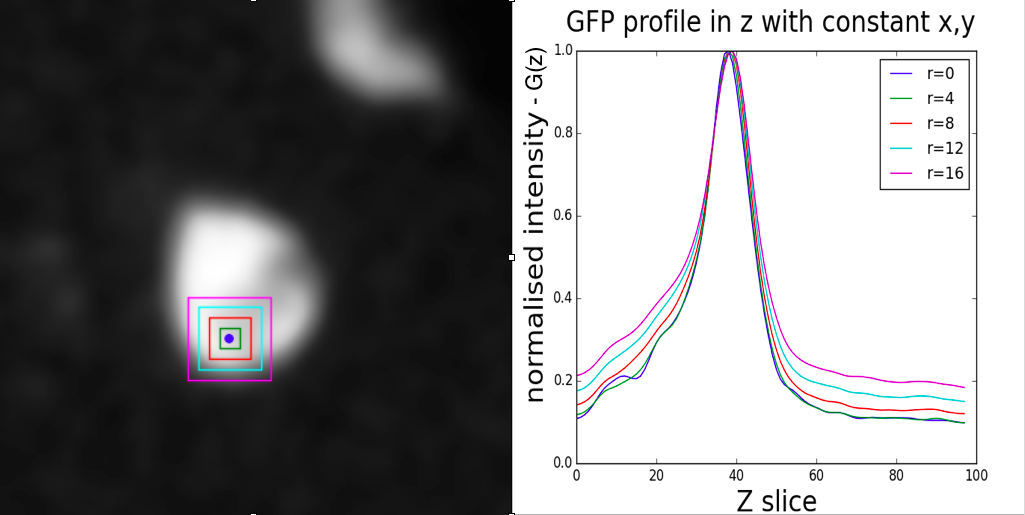
\includegraphics[width=0.9\textwidth]{401_gfp_profile}
 \caption{
 	GFP profile
 }
 \label{fig:gfpprofile}
\end{figure}

Similarly to the brightfield profile considered by Selinummi et al., measureable properties such as the variance, the location of the maximum value, and the mean value can be found for the GFP profile. The variance was found using the normalised profile, that is, the maximum value in each individual distribution is set to 1. Comparing profiles in an image can then be done using their mean value and variance. These are linearly related as shown in Figure [ref]. A background pixel will have a flat profile, giving a low variance and a high mean, since the majority of the distribution stays close the maximum value. As peaks appear in the profile due to the presence of objects, the mean will decrease, but the variance will increase proportionally. In this way, pixels with varying profile strengths can show very clearly whether they contain an object. Figure [ref] also shows a collections of blue points indicating points manually chosen to be inside cells. These are clustered in the high variance - low mean portion of the plot. The large cluster of points at low variance represent background pixels.

\begin{figure}[p]
 \centering
 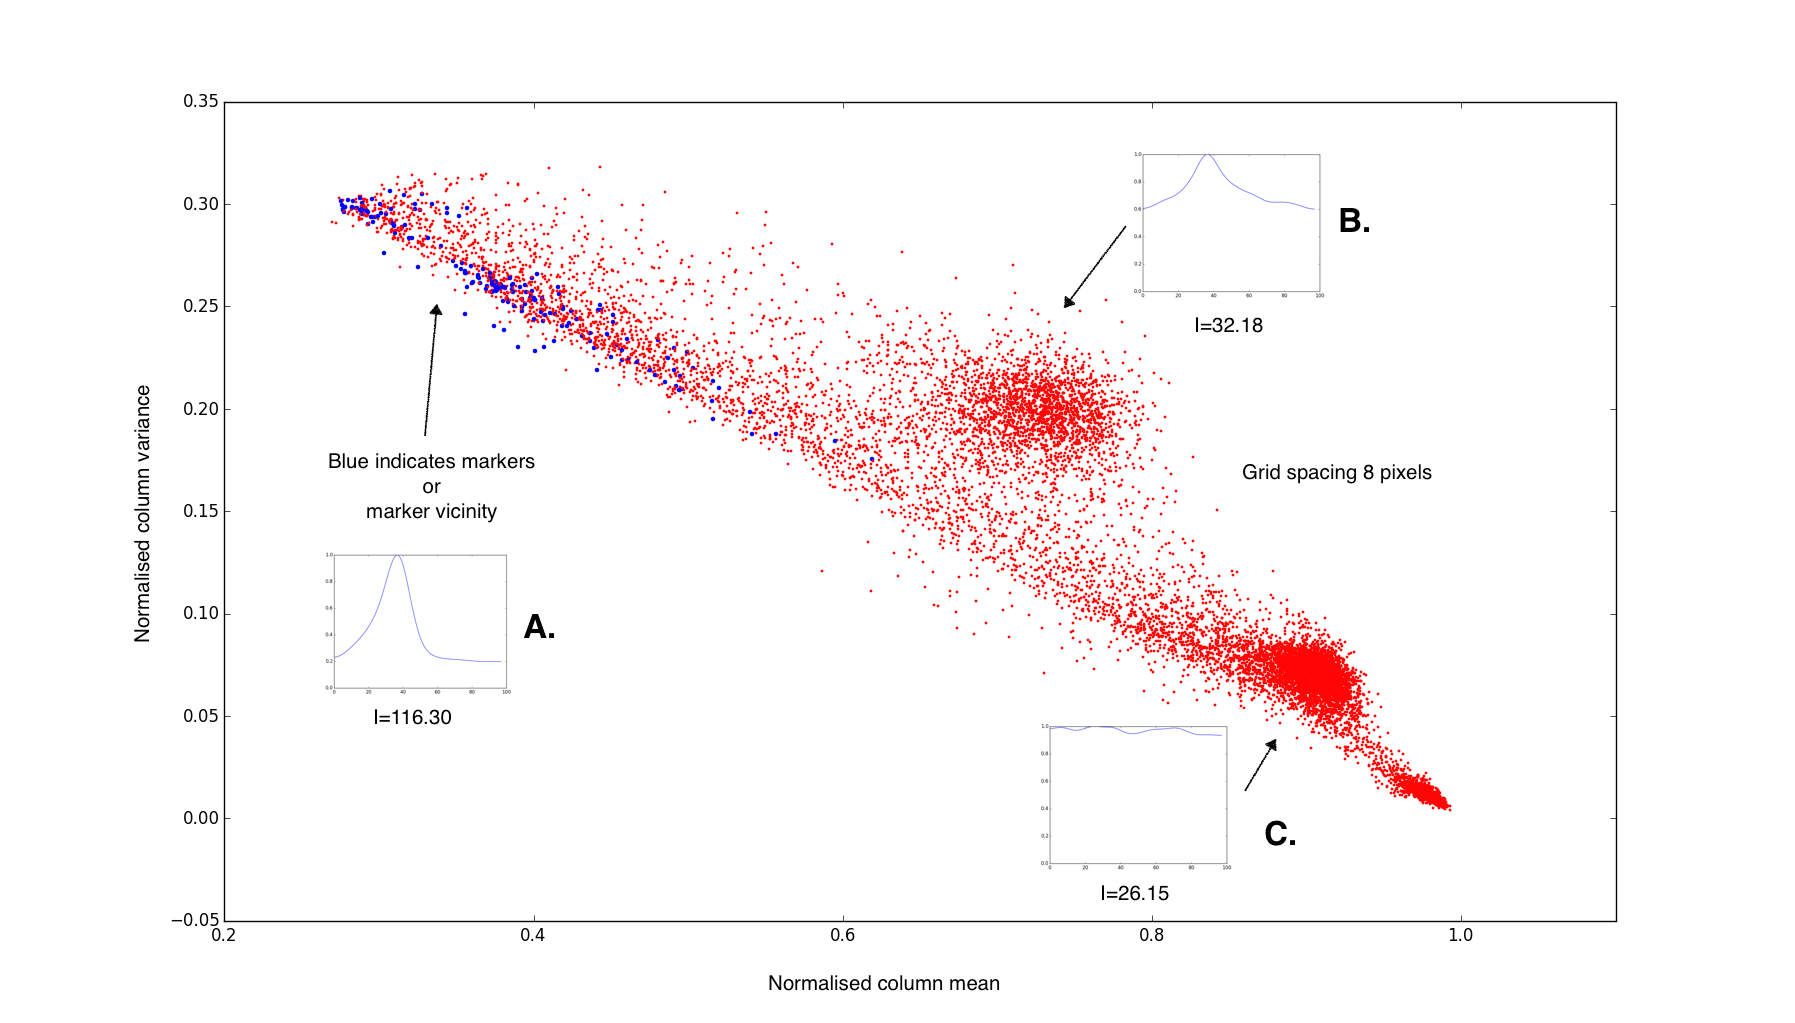
\includegraphics[width=0.9\textwidth]{402_gfp_scatter}
 \caption{
 	GFP scatter
 }
 \label{fig:gfpscatter}
\end{figure}

The most important part of the profile for the main method is the Z position of the maximum value. This indicates the peak intensity in the profile, and points to the most likely Z position of the part of the cell that contains the pixel in XY. This value can be used to search in the brightfield for an accurate cell representation by looking at the same level for the object in focus. Since the level indices are integers, the Z image was chosen by rounding the estimate of the Z position from the profile to the nearest integer. The more precise information is lost in the final image, but it can be stored elsewhere for further use.

\section{Optimum features for cell recognition}

By searching the brightfield with the GFP profile, the goal is to find the optimum features for segmentation. These include bright, smooth, uniformally coloured interiors surrounded by consistent, dark edges. Given a series of focal planes showing the object, it is likely that there is a single plane that contains the closest possible features to the ideal features required. This is assumed to be where the maximum GFP occurs. Unfortunately, the location of the maximum GFP for a cell shows an image that is ironically ``too focussed". When in the sharpest possible focus, a cell's edges become very thin and bright. To provide a better image for segmentation, a constant value is added to the level determined by the GFP profile. This was determined empirically and set to be between 4-8 levels added to the profile estimate. This is the second parameter for the method and is given the symbol $\Delta Z$.

For manual tracking, the accurate shape of the cell does not need to be known; it is better to see the interior of the cell clearly in order to make a good estimate of the centre to place a marker. The focal plane best for this type of observation also does not lie on plane with the maximum GFP. This shift is also empirically determined and is between 10-12 levels above the maximum GFP. This parameter is not crucial to the outcome of the method and is set by personal preference of the user tasked with finding the cells.

\begin{figure}[p]
 \centering
 \includegraphics[width=0.9\textwidth]{403_deltaz}
 \caption{
 	Delta Z
 }
 \label{fig:deltaz}
\end{figure}

\section{zMod and zBF}

For each frame in time, the Z position of the maximum of the GFP profile is calculated for each pixel in XY. A new image is created, called ``zMod", where the value of each pixel proportionally represents a Z position in the environment. This is analogous to a terrain. The range of values lies between 0 and 1, but the intermediate values are discretised to multiples of $\frac{1}{numberOfZPlanes}$ in order to represent the full Z range of the experiment. Floating point representation is easier to keep track of than integer representation in an image since the float value also works as a percentage height in the environment. This map of Z positions can be smoothed to make transitions between levels more gradual. The smoothing applied used a Gaussian blur with a radius of 3 pixels. This is the third important parameter and is given the symbol $\Sigma$.

\begin{figure}[p]
 \centering
 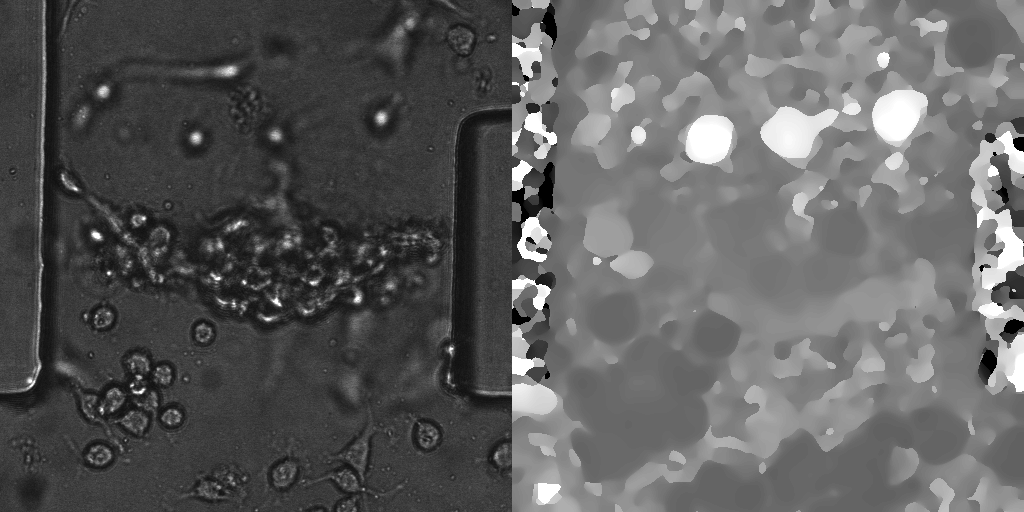
\includegraphics[width=0.9\textwidth]{403_zmod_example}
 \caption{
 	GFP profile
 }
 \label{fig:zmodexample}
\end{figure}

The zMod image for each frame can be mapped to the entire set of brightfield data for the same frame by selecting a pixel value from the brightfield stack focal plane that corresponds to the Z index indiciated by the zMod image. This produces the most important result of this study, the ``zBF" image. It is a single 2D image for each frame containing representations of all objects in focus with clear edges and interiors. This works by only selecting pixel values from the levels where the objects are in focus. This does not correct the focus of objects not marked by the GFP. This image is used to segment all cells in the environment simultaneously independently of their level in the experiment using 2D segmentation techniques.

\begin{figure}[p]
 \centering
 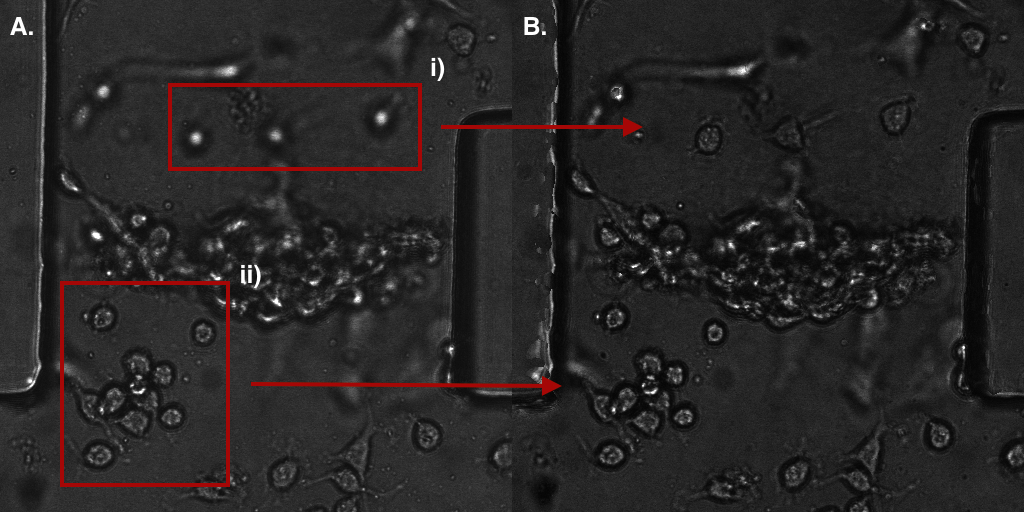
\includegraphics[width=0.9\textwidth]{404_zbf_example}
 \caption{
 	zBF side-by-side with brightfield
 }
 \label{fig:zbf}
\end{figure}

\section{Artificial edges for segmentation: zVar and zEdge}

A further improvement can be made to the segmentation. Part of the 3D data has already been used to correct the focus of objects marked with GFP. The part of the 3D data not used for this method is the mean (or equivalently the variance due to the linear relationship). This can indicate presence of an object more reliably than the absolute value of the GFP. Pixels with very different values in the GFP can have similar values in the mean image since the profiles are normalised such that only the shape of the distribution matters. If the mean of the normalised and inverted (since low mean/high variance indicates an object) GFP profile for each pixel in a frame is found, a new image, ``zVar" can be made. Depending on the linear smoothing of the original data (the parameter $R$), the boundary of objects in the mean image can extend beyond the edges of objects in the brightfield.

\begin{figure}[p]
 \centering
 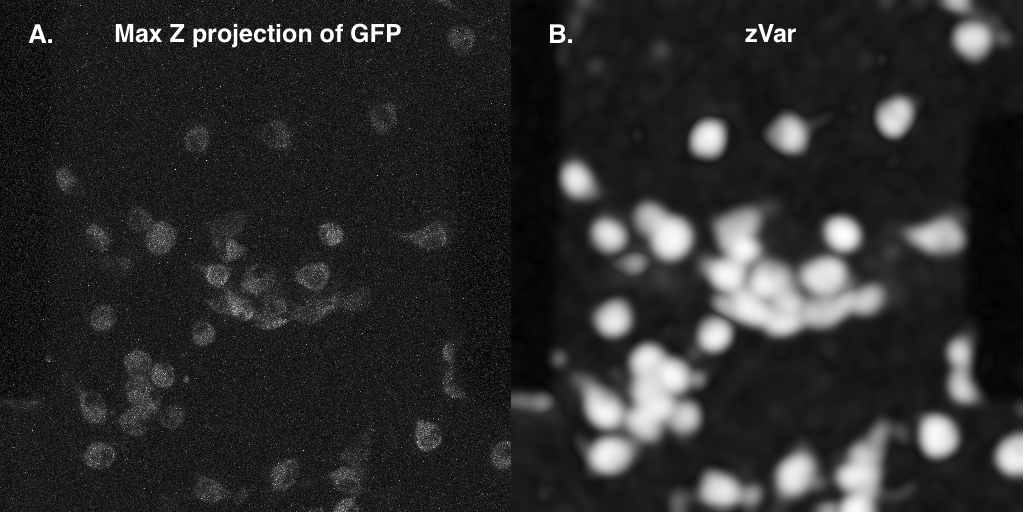
\includegraphics[width=0.9\textwidth]{405_zvar}
 \caption{
 	zVar
 }
 \label{fig:zvar}
\end{figure}

The extra extent of the zVar image is exploited to provide a maximum boundary for segmentation, this is combined with zMod to produce outlines around cells. This does not require the edges to be followed correctly, but only needs to enclose the general shape of the cell. These shapes are then segmented to separate objects or even rough groups of objects. The outlines of the segmentation are used to generate artificial edges using a DoF (Difference of Gaussians) edge model. These edges cut through background values that are similar in intensity to the interiors of cells. If there is a gap in the cell edge with an intensity close to the background, the segmentation will expand into the background and cause a major overestimation of the area of the cell. This image is called ``zEdge" and is the image for each frame used to provide the final segmentation data for each experiment.

\begin{figure}[p]
 \centering
 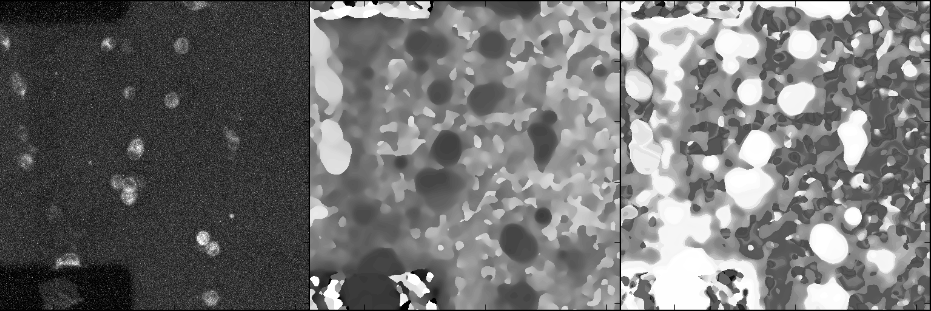
\includegraphics[width=0.9\textwidth]{406_zunique}
 \caption{
 	zUnique
 }
 \label{fig:zunique}
\end{figure}

\begin{figure}[p]
 \centering
 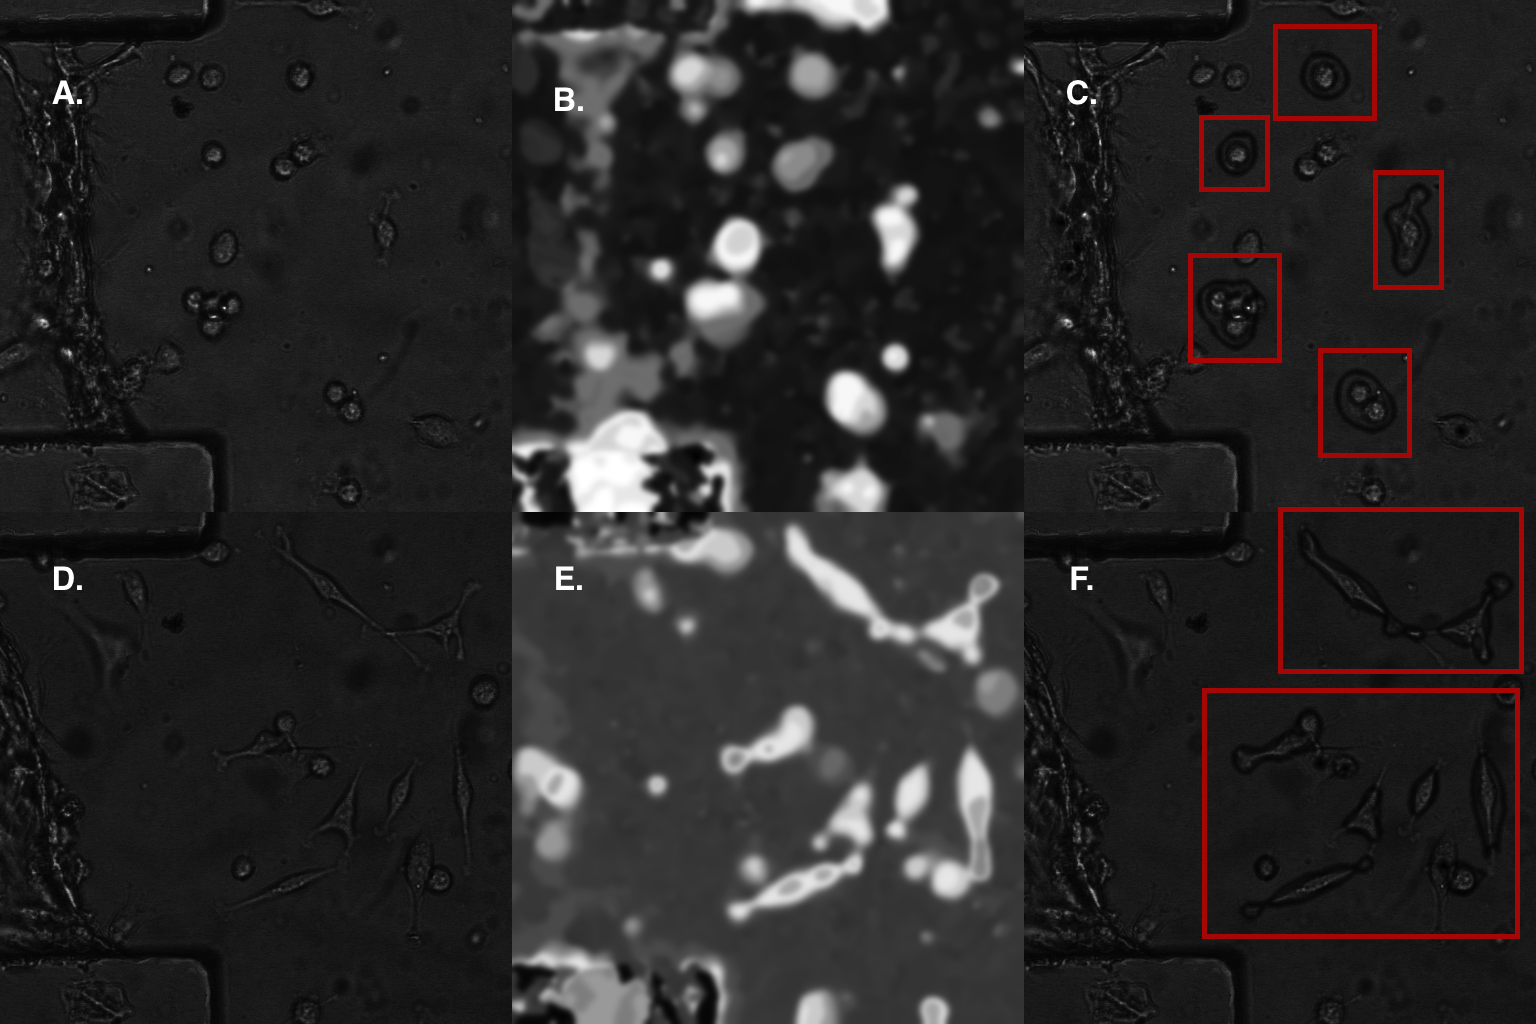
\includegraphics[width=0.9\textwidth]{407_zedge}
 \caption{
 	zEdge
 }
 \label{fig:zedge}
\end{figure}

\section{Protrusion measurement}

One of the main aims of this study is to accurately measure the lengths and orientations of the cell protrusions to gather useful data on cell behaviour. The protrusions were measured by plotting the outline of the cell on a polar graph and measuring the divergence from a smooth circular shape as measured from the calculated cell centre. The protrusions show as peaks in this plot and their length is measured from the tip of the peak to the mean radius, not the centre of the cell.

\begin{figure}[p]
 \centering
 \includegraphics[width=0.9\textwidth]{408_protrusions_calculation}
 \caption{
 	Protrusion calculation
 }
 \label{fig:protrusioncalc}
\end{figure}

\section{Summary of the method}

To summarise the steps taken to pre-process 3D image data for segmentation:
\begin{enumerate}
\item Smooth the data to reduce noise.
\item For each pixel in XY for the 3D data, find the vertical intensity distribution in Z, or ``profile", for each pixel nd evaluate its properties.
\item Using the profile for each pixel, create an image where the value of a pixel is proportional to the Z level of the maximum intensity of GFP at that XY location. This is zMod.
\item For zMod, there are three parameters that must be chosen: $R$, the radius of the linear smoothing kernel, which affects only the GFP in XY; $\Delta Z$, the vertical shift to locate the ideal edges for segmentation; and $\Sigma$, the size of the gaussian smoothing kernel, which affects the GFP in Z.
\item Map the Z values in zMod to the stack of image data for the brightfield. Select pixel values from the brightfield whose Z level corresponds to that indicated by zMod and place them into a new image, called zBF.
\item Although zBF now contains in-focus representations of each object marked with GFP, a further improvement can be made using the outlines of the GFP mean image. The mean image, zVar, takes the mean value of the normalised GFP profile as the value of each pixel. This gives a maximum extent of the cell and limits segmentation to a boundary to prevent it from extending into the background and incorrectly judging the area of a cell.
\item The final image, zEdge, is prepared for segmentation by using the zVar and edges of regions in zMod to automatically draw edges on the image that follow a similar edge profile to the dark edges found in the zBF image. zEdge then contains the same information as zBF, but with bounding edges beyond which the segmentation cannot extend.
\item Finally, once segmentation is complete, cell properties such as project area can be obtained along with protrusion lengths and orientations. Protrusions are found by radially plotting the distance of the edge from the centre point and designating outliers as protrusions.
\end{enumerate}

Figure [ref] below shows the full paradigm of the method.
\begin{figure}[p]
 \centering
 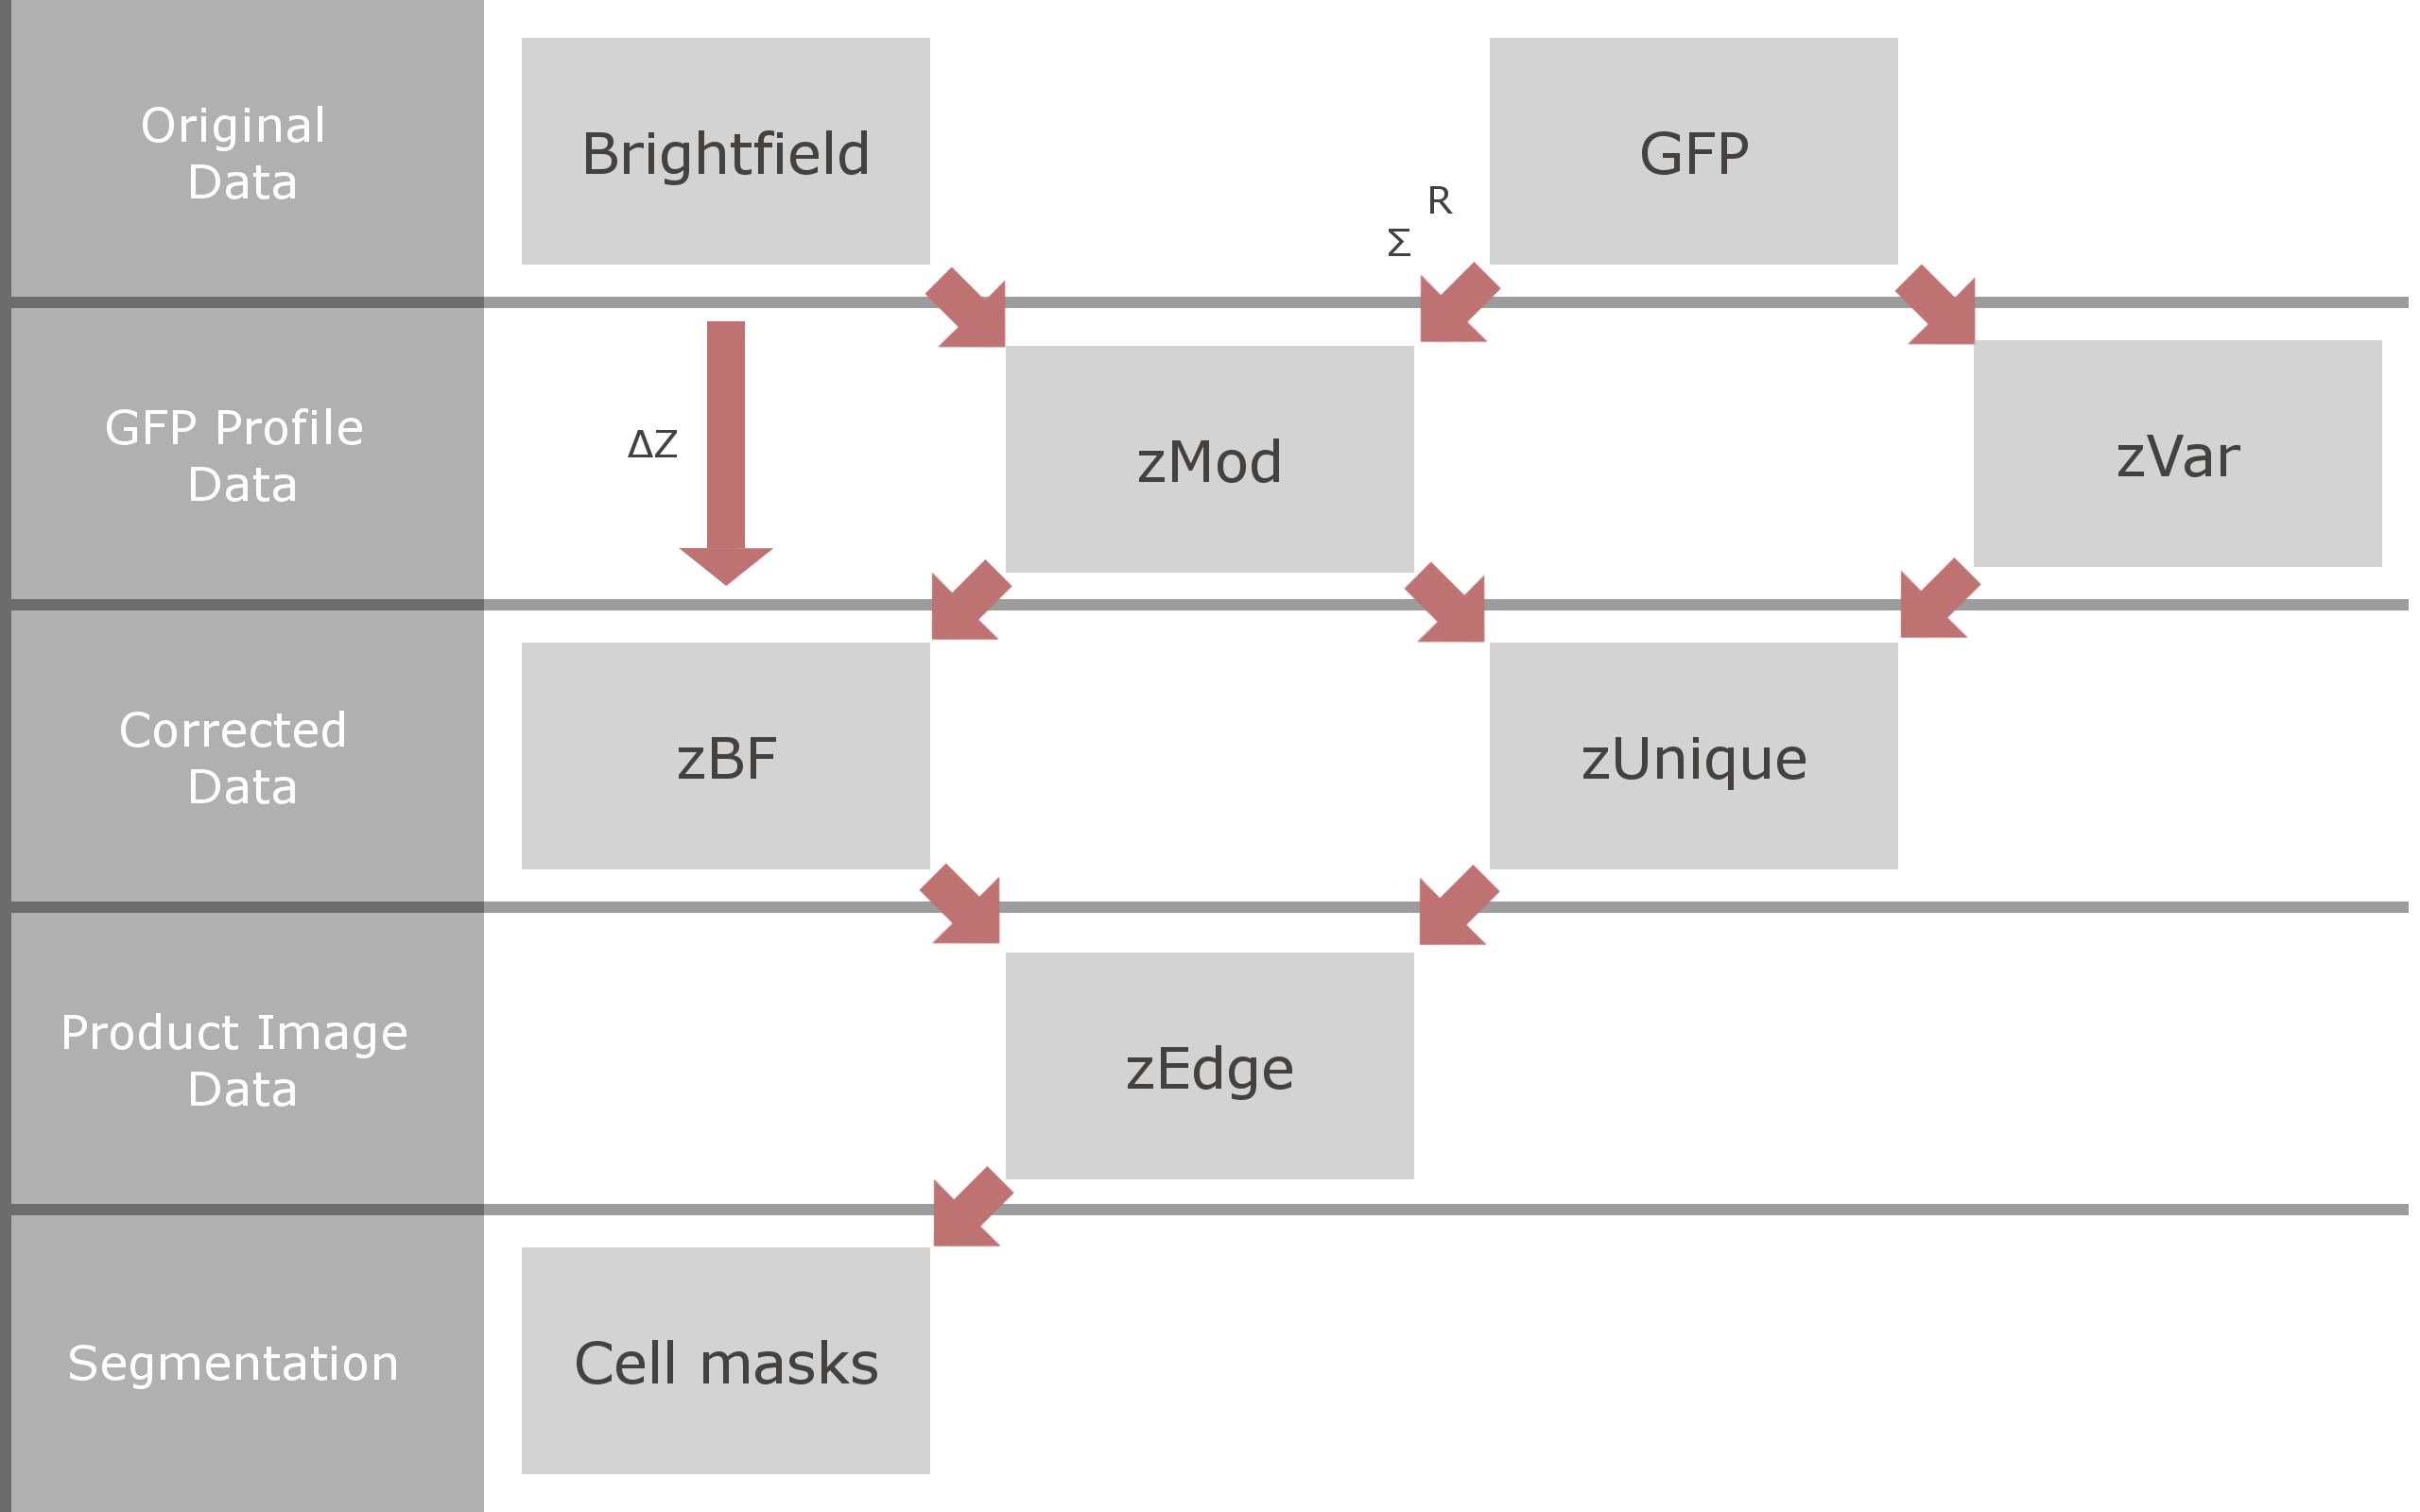
\includegraphics[width=0.9\textwidth]{409_method_flowchart}
 \caption{
 	Method flow chart
 }
 \label{fig:flowchart}
\end{figure}
